\documentclass[a4paper,oneside,10pt]{article}
\usepackage{wallpaper}
\usepackage{float}
\usepackage[utf8]{inputenc}
\usepackage{circuitikz}
\usepackage{listings}
\usepackage{indentfirst}
\lstdefinelanguage{Arduino}{
	language=C++,
	morekeywords={
		void,
		setup,
		loop,
		pinMode,
		digitalWrite,
		digitalRead,
		analogRead,
		analogWrite,
		delay,
		delayMicroseconds,
		millis,
		micros,
		SPI,
		Wire,
		Serial,
		HIGH,
		LOW,
		INPUT,
		OUTPUT,
		INPUT_PULLUP
	},
	morekeywords=[2]{
		SPIClass,
		SPISettings,
		begin,
		end,
		transfer,
		transfer16,
		beginTransaction,
		endTransaction
	},
	sensitive=true
}
\lstdefinestyle{mystyle}{
	columns=fullflexible,
	frame=single,
	breaklines=true,
	numbers=left,
	tabsize=2,
	belowcaptionskip=1\baselineskip,
	language=Arduino,
	showstringspaces=false,
	basicstyle=\footnotesize\ttfamily,
	keywordstyle=\bfseries\color{green!40!black},
	commentstyle=\itshape\color{purple!40!black},
	identifierstyle=\color{blue},
	stringstyle=\color{orange},
	keywordstyle=[2]\bfseries\color{green!40!black},
	literate=
	{á}{{\'a}}1
	{é}{{\'e}}1
	{í}{{\'i}}1
	{ó}{{\'o}}1
	{ú}{{\'u}}1
	{à}{{\`a}}1
	{â}{{\^a}}1
	{ê}{{\^e}}1
	{ô}{{\^o}}1
	{ã}{{\~a}}1
	{õ}{{\~o}}1
	{ç}{{\c{c}}}1
	{Á}{{\'A}}1
	{É}{{\'E}}1
	{Í}{{\'I}}1
	{Ó}{{\'O}}1
	{Ú}{{\'U}}1
	{À}{{\`A}}1
	{Â}{{\^A}}1
	{Ê}{{\^E}}1
	{Ô}{{\^O}}1
	{Ã}{{\~A}}1
	{Õ}{{\~O}}1
	{Ç}{{\c{C}}}1
}
\lstset{style=mystyle}
\renewcommand{\lstlistingname}{Código}
\usepackage{graphicx}
\usepackage[alf]{abntex2cite}
\usepackage{hyphenat}
\usepackage[brazil]{babel}
\setlength{\textwidth}{16cm} %
\setlength{\textheight}{23cm} %
\setlength{\oddsidemargin}{0cm} %
\setlength{\evensidemargin}{0cm} %
\setlength{\topmargin}{0cm}
\CenterWallPaper{1.01}{bg.pdf}

\begin{document}

\noindent Relatório 5: Comunicação SPI. \\
Internet das Coisas - Integral\\
Prof. Gabriel de Freitas Fernandes\\
2026.2\\
\\
\textbf{EQUIPE:} \\ Arthur Peixoto - 170.214 \\ Gabriel Oliva Gurgel - 168.860 \\ Guilherme Samuel dos Santos - 168.867

\section{Introdução}
Um dos protocolos mais difundidos para comunicação serial é o \textbf{Serial Peripheral Interface (SPI)}. Trata-se de uma especificação voltada para uma interface onde ocorre comunicação serial síncrona, destinada principalmente à comunicação de curta distância entre dispositivos. O protocolo permite a transmissão de dados em modo \textit{full duplex} e, em sua configuração tradicional, adota uma arquitetura \textit{master-slave}, na qual um único dispositivo atua como mestre (\textit{master}) e os demais como escravos (\textit{slaves}).

Nesta prática, será realizada uma atividade introdutória de comunicação entre dois microcontroladores ESP32, sendo um configurado como dispositivo mestre e o outro como dispositivo escravo. Além da implementação prática da comunicação utilizando o protocolo SPI, serão revisados conceitos fundamentais relacionados ao funcionamento do protocolo, por meio de um estudo baseado na documentação dos dispositivos e nos conteúdos apresentados em aula.
\section{Revisão de conceitos}

\subsection{Funções relevantes}
A biblioteca \texttt{SPI.h} já está incluída no ambiente de desenvolvimento, portanto, não foi necessário realizar sua instalação separadamente \cite{arduino}. Aqui estão informações sobre as principais funções relacionadas ao SPI usadas:

\subsubsection{Interface SPI nativa}
\begin{itemize}
	\item \texttt{SPI.begin()}: inicializa o barramento SPI, configurando os pinos SCK (também conhecido como \textbf{Serial Clock}, ou apenas \textbf{Clock} - sigla \textbf{CLK}), MOSI e SS como saídas (com SCK e MOSI em nível baixo e SS em nível alto) e o pino MISO como entrada. Após chamar essa função, o dispositivo opera como controlador no barramento SPI. Não possui retorno nem parâmetros.
	\item \texttt{SPISettings()}: é utilizado para configurar a porta SPI para um dispositivo SPI específico. Ele combina três parâmetros (velocidade do clock, ordem dos bits e modo de dados) em um único objeto, a proporcionar maior organização e clareza durante a configuração e a etapa inicial de \textit{setup}. Essa função não possui valor de retorno. \\ Os parâmetros são:
	\begin{itemize}
		\item \texttt{speedMaximum}: a velocidade máxima de clock em \textit{Hz} (hertz). Por exemplo, podemos usar um \texttt{int} de \texttt{20000000} para um periférico com especificação de até 20 MHz.
		\item \texttt{dataOrder}: a ordem dos bits para transferência de dados. Os valores permitidos são \texttt{MSBFIRST} (bit mais significativo é enviado por primeiro) e \texttt{LSBFIRST} (bit menos significativo é enviado por primeiro).
		\item \texttt{dataMode}: o modo de dados SPI. os valores permitidos são \texttt{SPI\_MODE0}; \texttt{SPI\_MODE1}; \texttt{SPI\_MODE2}; e \texttt{SPI\_MODE3}.
	\end{itemize}
	\item \texttt{SPI.beginTransaction()}: configura o barramento SPI com as definições especificadas e assume o controle exclusivo do mesmo. Esta função deve ser chamada antes de se comunicar com um periférico SPI específico, para garantir a configuração correta e evitar conflitos com outros dispositivos SPI ou interrupções. Por padrão, \texttt{SPI.begin()} deve ser chamado antes de utilizar esta função. Não possui retorno e possui um parâmetro chamado \texttt{mySettings}, onde é necessário chamar um objeto do tipo \texttt{SPISettings()} em que é selecionado as configurações de SPI a serem aplicadas.
	\item \texttt{SPI.transfer()}: realiza uma operação simultânea de envio e recebimento de dados por meio do barramento SPI. Isso ocorre em razão de o SPI ser um protocolo \textbf{full-duplex}, no qual a transmissão e a recepção de dados são realizadas simultaneamente durante a comunicação.
	A função não possui valor de retorno e recebe dois parâmetros: \texttt{val} (ou \texttt{buffer}), responsável por especificar o dado ou conjunto de dados a ser transmitido, e \texttt{size}, que define a quantidade de bytes a serem transferidos. Dessa forma, é possível realizar a transmissão de um único byte ou de um conjunto de bytes, quando fornecido um arranjo (\textit{array}). Por padrão, o parâmetro \texttt{size} assume o valor correspondente a 1 byte.
\end{itemize}
\subsubsection{Interface proprietária da Espressif}
\begin{itemize}
	\item \texttt{spi\_slave\_initialize()}: inicializa a interface SPI no modo \textit{slave}, configurando o barramento e os parâmetros específicos do dispositivo. A função recebe quatro parâmetros:
	\begin{itemize}
		\item \texttt{host}: que identifica o periférico SPI a ser utilizado;
		\item \texttt{bus\_config}, que contém as configurações dos pinos e do barramento; \texttt{slave\_config}, que define as configurações específicas do dispositivo \textit{slave};
		\item \texttt{dma\_chan}, que determina o canal de DMA (\textit{Direct Memory Access}, onde o próprio periférico se encarregará da leitura e processamento, liberando a CPU de quase todo o processamento antes necessário) utilizado. Neste código, é utilizado o periférico \texttt{VSPI\_HOST}, os endereços das estruturas \texttt{busConfig} e \texttt{slaveConfig}, e \texttt{SPI\_DMA\_DISABLED}, indicando que a transferência por DMA não será utilizada. A função retorna um valor do tipo \texttt{esp\_err\_t}, utilizado para indicar se a inicialização foi realizada com sucesso ou se ocorreu algum erro.
	\end{itemize}
	\item \texttt{spi\_slave\_transmit()}: realiza uma transação SPI no modo \textit{slave}, aguardando que o controlador inicie a comunicação e realize a transferência dos dados. A função recebe três parâmetros:
	\begin{itemize}
		\item \texttt{host}: identifica o periférico SPI utilizado;
		\item \texttt{trans\_desc}: é um ponteiro para uma estrutura do tipo \texttt{spi\_slave\_transaction\_t} contendo as informações da transação, como o tamanho dos dados e o \textit{buffer} de recepção;
		\item \texttt{ticks\_to\_wait}: define por quanto tempo a função deve aguardar pela realização da transação.
	\end{itemize}  
	No código, é utilizado \texttt{portMAX\_DELAY}, permitindo que o dispositivo aguarde indefinidamente até que o controlador inicie a comunicação. A função retorna um valor do tipo \texttt{esp\_err\_t}, sendo possível verificar, por exemplo, se a operação foi concluída com sucesso por meio da comparação com \texttt{ESP\_OK}.
\end{itemize}
\newpage
\subsection{Comparação entre UART e SPI (benefícios e malefícios)}

\begin{table}[h]
	\centering
	\setlength{\tabcolsep}{10pt}
	\renewcommand{\arraystretch}{2}
	\small
	\begin{tabular}{|l|p{5.5cm}|p{5.5cm}|}
		\hline
		\textbf{Critério} & \textbf{\nohyphens{Universal Asynchronous Receiver/Transmitter (UART)}} & \textbf{Serial Peripheral Interface (SPI)} \\
		\hline
		Tipo de comunicação & Assíncrona (dispositivos podem operar com clocks internos independentes). & Síncrona (precisa de um clock dedicado). Elimina problemas relacionados a desalinhamento de taxa. \\
		\hline
		Barramento & Apenas dois fios são o suficiente (\textbf{TX} e \textbf{RX}). & No mínimo, 4 fios (Clock, MOSI, MISO, CS) \\
		\hline
		Topologia & Ponto a ponto (1 mestre - 1 dispositivo) & Mestre com múltiplos escravos (1 CS por escravo). \\
		\hline
		Velocidade típica & Baixa a moderada (até aproximadamente 1 Mbps) & Alta (dezenas de Mbps) \\
		\hline
		Configuração & Taxa de transmissão (conhecido como \textit{baud rate }) deve ser igual em ambos os lados & Apenas configuração de modo de clock (alto ou baixo) \\
		\hline
		Transmissão & Bits de start/stop e paridade opcional & Mínimo, sem bits extras por byte \\
		\hline
		Escalabilidade & Difícil escalar para múltiplos dispositivos & Fácil, basta adicionar mais linhas CS \\
		\hline
		Detecção de erro & Paridade opcional & Nenhuma nativa \\
		\hline
		Distância de uso & Maior alcance (ex.: RS-232, RS-485) & Curta distância (dentro da placa) \\
		\hline
		Complexidade& Geralmente é mais simples & Geralmente é mais complexo (ex.: gerenciamento de CS e modos) \\
		\hline
	\end{tabular}
	\caption{Comparação direta entre comunicação UART e SPI}
	\label{tab:uart_spi}
\end{table}
\newpage
\section{Prática}

\subsection{Montagem Experimental}

O ESP32 dispõe de quatro periféricos de comunicação SPI, denominados \textbf{SPI0}, \textbf{SPI1}, \textbf{HSPI} e \textbf{VSPI}, segundo a sua documentação oficial de programação. Para a realização da prática, foi adotada a interface \textbf{VSPI}, pois foi a configuração inicialmente definida pelo grupo. Não foi necessário testar outra maneira de ligação.

\begin{figure}[H]
	\centering
	\begin{minipage}[b]{0.4\textwidth}
		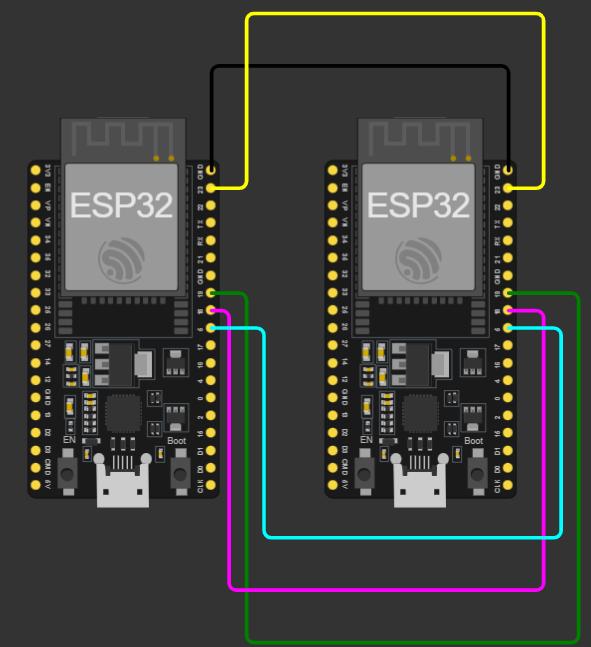
\includegraphics[width=\textwidth]{s1}
		\caption{Simulação das entradas}
	\end{minipage}
	\hfill
	\begin{minipage}[b]{0.4\textwidth}
		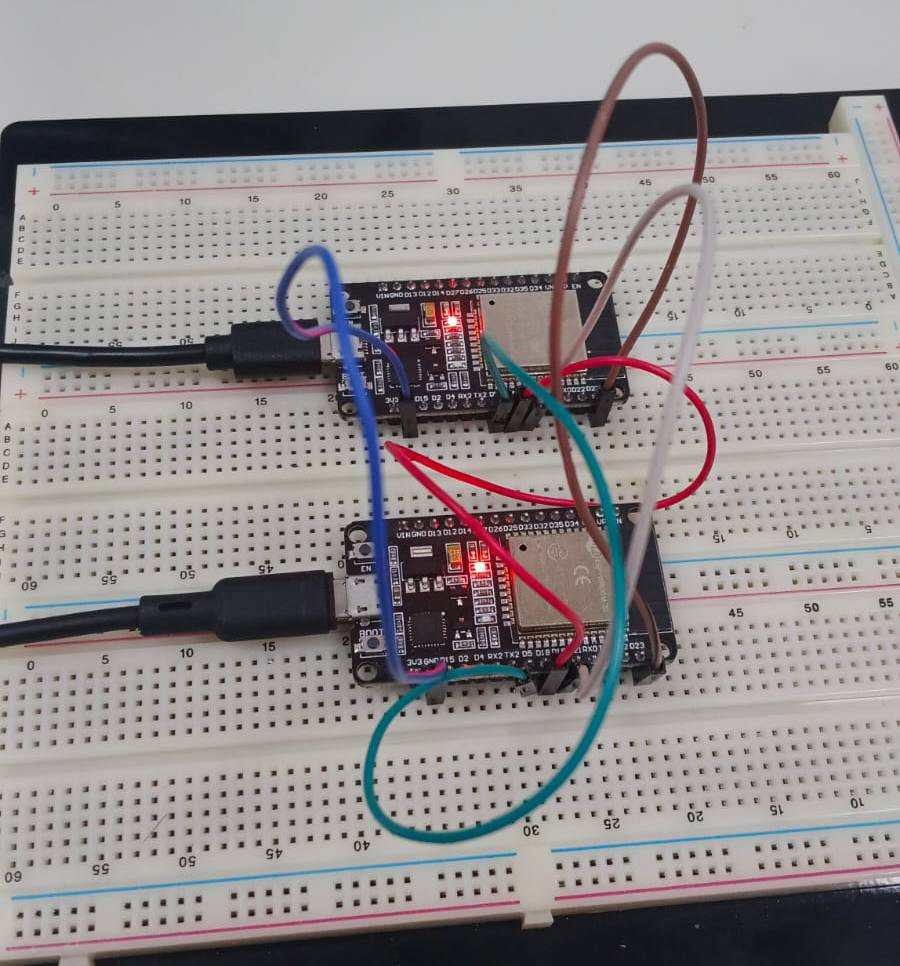
\includegraphics[width=\textwidth]{original}
		\caption{Montagem do circuito feita no laboratório}
	\end{minipage}
\end{figure}

\begin{figure}[H]
	\begin{circuitikz}[american, scale=1.15, every node/.style={transform shape}]
	
	\draw[thick] (0,0) rectangle (3,6);
	\node[font=\bfseries] at (1.5,6.5) {ESP32 (Master)};
	
	\draw[thick] (10,0) rectangle (13,6);
	\node[font=\bfseries] at (11.5,6.5) {ESP32 (Slave)};
	
	\node[anchor=east, font=\footnotesize] at (2.9,5) {GPIO23 (MOSI)};
	\draw (3,5) -- (3.5,5);
	
	\node[anchor=east, font=\footnotesize] at (2.9,4) {GPIO19 (MISO)};
	\draw (3,4) -- (3.5,4);
	
	\node[anchor=east, font=\footnotesize] at (2.9,3) {GPIO18 (SCK)};
	\draw (3,3) -- (3.5,3);
	
	\node[anchor=east, font=\footnotesize] at (2.9,2) {GPIO5 (SS)};
	\draw (3,2) -- (3.5,2);
	
	\node[anchor=east, font=\footnotesize] at (2.9,1) {GND};
	\draw (3,1) -- (3.5,1);
	
	\node[anchor=west, font=\footnotesize] at (10.1,5) {GPIO23 (MOSI)};
	\draw (10,5) -- (9.5,5);
	
	\node[anchor=west, font=\footnotesize] at (10.1,4) {GPIO19 (MISO)};
	\draw (10,4) -- (9.5,4);
	
	\node[anchor=west, font=\footnotesize] at (10.1,3) {GPIO18 (SCK)};
	\draw (10,3) -- (9.5,3);
	
	\node[anchor=west, font=\footnotesize] at (10.1,2) {GPIO5 (SS)};
	\draw (10,2) -- (9.5,2);
	
	\node[anchor=west, font=\footnotesize] at (10.1,1) {GND};
	\draw (10,1) -- (9.5,1);
	
	\draw[thick] (3.5,5) -- (9.5,5) node[midway, above, font=\footnotesize\bfseries] {MOSI};
	\draw[thick] (3.5,4) -- (9.5,4) node[midway, above, font=\footnotesize\bfseries] {MISO};
	\draw[thick] (3.5,3) -- (9.5,3) node[midway, above, font=\footnotesize\bfseries] {SCK};
	\draw[thick] (3.5,2) -- (9.5,2) node[midway, above, font=\footnotesize\bfseries] {SS / CS};
	\draw[thick] (3.5,1) -- (9.5,1) node[midway, above, font=\footnotesize\bfseries] {GND};
	
	\end{circuitikz}
	\caption{Esquema das entradas}
\end{figure}

\subsection{Código}

Para o \textit{master}, chegamos a usar primeiramente um valor de 70 MHz, visto que a interface de SPI do ESP32 consegue transmitir até no máximo, aproximadamente 80 MHz \cite{espressifSPI}. Todavia, resolvemos diminuir drasticamente a frequência com o objetivo de evitar saídas inconsistentes no Monitor Serial, além de termos maior certeza que o byte foi transmitido. Assim, para padronização, definimos um valor de 15MHz.

Em relação a comunicação serial USB entre os controladores e o ambiente de desenvolvimento do computador, usamos um \textit{baud rate} de \texttt{9600}, por ser o valor que estamos usando nas aulas, apesar da documentação usar \texttt{115200}. A convenção de colocar o SS em pino alto para parar a transmissão, e pino baixo para iniciar vem do modo 0 do SPI, definido no último argumento do objeto \texttt{SPISettings}. 
\newline

\lstinputlisting[caption=Código do controlador \textit{master}]{esp32_spi_master.ino}

A implementação do código do \textit{slave} veio inicialmente reutilizamos a mesma lógica empregada no \textit{master}, considerando a característica do protocolo SPI de realizar a comunicação em \textit{full-duplex}, permitindo o envio e o recebimento de dados simultaneamente. Entretanto, essa abordagem de usar o mesmo \texttt{SPI.transfer()} não apresentou o funcionamento esperado, uma vez que não foram observados resultados realmente efetivos de transmissão durante o monitoramento da comunicação, apenas bytes aleatórios inconclusivos. 

Após novas pesquisas e análises da documentação, optamos pela utilização da \texttt{driver/spi\_slave.h}, que fornece recursos específicos para a configuração do ESP32 como um \textit{slave} no barramento. Um possível motivo, apontado por participantes do fórum da Espressif, é que a utilização genérica para implementar um dispositivo \textit{slave}, sem os recursos específicos citados, pode levar o dispositivo a tentar gerar seu próprio sinal de \textit{clock}. Como ele deve ser gerado exclusivamente pelo \textit{master}, caso ambos os dispositivos tentem controlar a transmissão de SCK, pode ocorrer um conflito elétrico, uma vez que, segundo os usuários: "essa linha normalmente opera em configuração \textit{push-pull}, podendo resultar em correntes superiores aos limites especificados."\cite{espressifSPISlave}
\newline
Portanto, foi possível implementar a comunicação utilizando diretamente os mecanismos disponibilizados pelo \textit{driver} específico para essa finalidade. Aqui é importante destacar as seguintes \textit{structs} (estruturas):

\begin{itemize}
	\item \texttt{spi\_bus\_config\_t}: estrutura utilizada para definir a configuração dos pinos e características do barramento SPI. No código, os campos \texttt{mosi\_io\_num}, \texttt{miso\_io\_num} e \texttt{sclk\_io\_num} são utilizados para especificar, respectivamente, os pinos MOSI, MISO e SCLK.
	\item \texttt{spi\_slave\_interface\_config\_t}: estrutura responsável por armazenar as configurações específicas da interface SPI no modo \textit{slave}. O campo \texttt{spics\_io\_num} define o pino utilizado pelo sinal CS (\textit{Chip Select}), enquanto \texttt{mode} determina o modo SPI utilizado na comunicação. Neste código, o valor \texttt{0} corresponde ao \texttt{SPI\_MODE0}. O campo \texttt{queue\_size} determina a quantidade máxima de transações que podem ser mantidas na fila, sendo configurado como \texttt{1} (um byte, não estamos enviando um \textit{array} em um \textit{buffer}).
	
	\item \texttt{spi\_slave\_transaction\_t}: estrutura utilizada para descrever uma transação SPI realizada pelo dispositivo \textit{slave}. No código, o campo \texttt{length} especifica o tamanho da transferência em bits, sendo configurado como \texttt{8}, correspondente a um byte. O campo \texttt{rx\_buffer} recebe o endereço da variável \texttt{data}, indicando o local da memória no qual os dados recebidos pelo \textit{slave} serão armazenados. Dessa forma, após a conclusão da transação, o byte recebido pelo dispositivo pode ser acessado por meio da variável \texttt{data}.
\end{itemize}

\lstinputlisting[caption=Código do controlador \textit{slave}]{esp32_spi_slave.ino}
\newpage
\subsection{Resultados e Discussão}

Foi possível verificar que a transmissão inicialmente realizada utilizava bytes fixos, como o \texttt{char} \texttt{'A'} ou o \texttt{int} \texttt{65}.

\begin{figure}[H]
	\centering
	\begin{minipage}[b]{0.4\textwidth}
		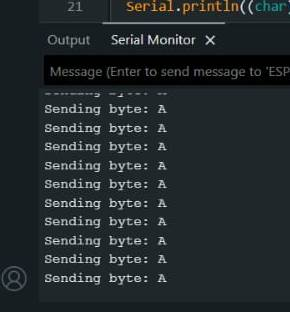
\includegraphics[width=\textwidth]{result_master}
		\caption{Monitoramento serial no \textit{master}}
	\end{minipage}
	\hfill
	\begin{minipage}[b]{0.4\textwidth}
		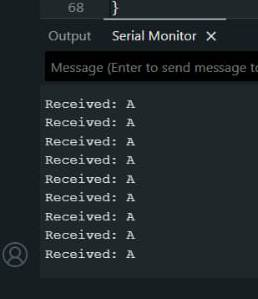
\includegraphics[width=\textwidth]{result_slave}
		\caption{Monitoramento serial no \textit{slave}}
	\end{minipage}
\end{figure}

Para realizar testes mais abrangentes, optamos por utilizar a função \texttt{Serial.read()} no código-fonte do \textit{master}, permitindo verificar a transmissão de diferentes bytes e de \textit{strings}, ao digitar pelo teclado do computador. Os testes também foram realizados com sucesso, confirmando o funcionamento da comunicação para diferentes tipos de dados.

\subsection{Verificação com Osciloscópio}

\begin{figure}[H]
	\centering
	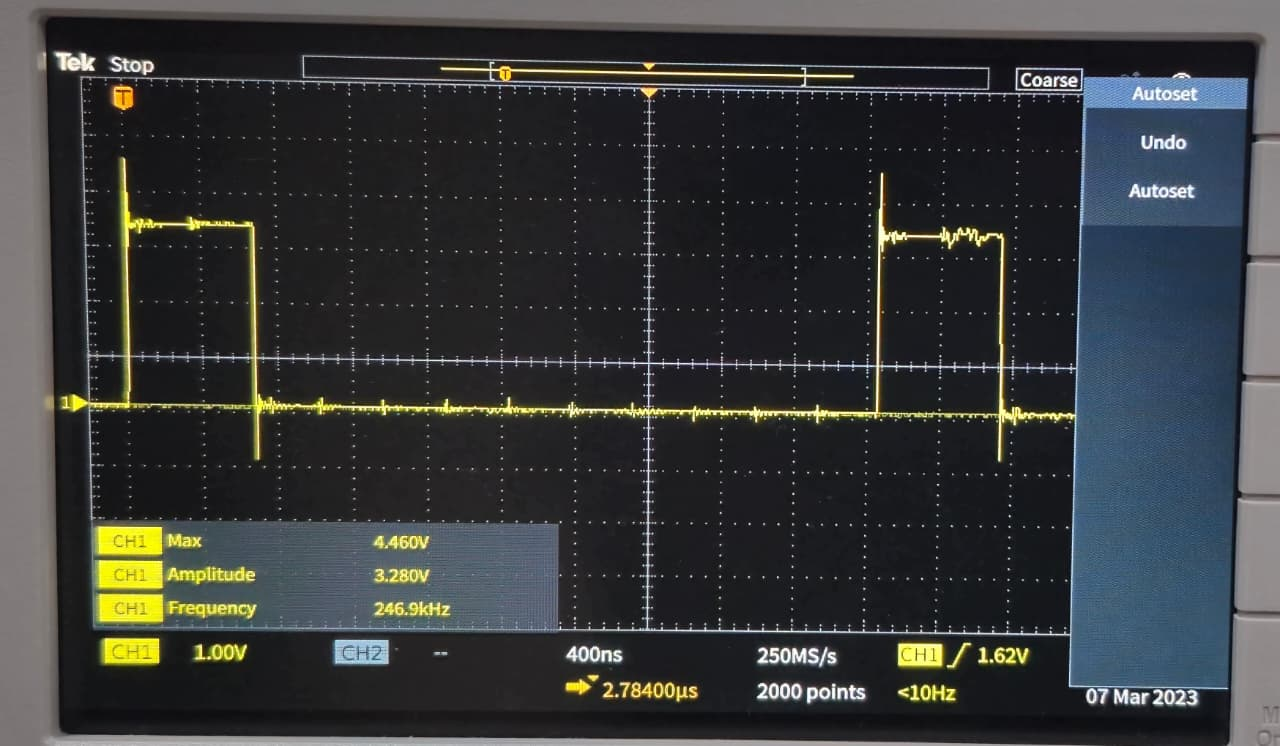
\includegraphics[scale=0.2]{oscilloscope}
	\caption{Estado do barramento CS visto em detalhes}
\end{figure}

Por meio do monitoramento com o osciloscópio, foi possível observar um pouco do comportamento do sinal de CS, e seu comportamento durante a transmissão. Na Figura 6, o pino CS permanece em nível baixo enquanto o byte é transmitido, intervalo que corresponde a cerca de 8 pulsos de clock, um para cada bit. A subida do sinal para nível alto indica o término da transmissão, após o qual o algoritmo do mestre aguarda 1 segundo (\textit{delay}) antes do envio seguinte.

\subsubsection{Comunicação entre ESP32 e outros dispositivos}

Agora que foi possível estabelecer a comunicação entre dois ESP32, podemos analisar algumas características relacionadas à quantidade de dispositivos simultâneos no SPI. Caso seja necessário conectar vários ao mesmo controlador, as linhas MOSI, MISO e SCK podem ser compartilhadas entre todos os dispositivos, enquanto cada dispositivo deve possuir uma forma individual de seleção por meio do CS. Durante uma transferência de bytes, somente o dispositivo selecionado deve habilitar sua saída na linha MISO, enquanto os demais permanecem desabilitados. No caso da configuração utilizada neste relatório, o dispositivo é selecionado quando o sinal CS é colocado em nível baixo.
\par
Essa característica faz com que a quantidade de dispositivos conectados diretamente ao barramento seja limitada principalmente pela quantidade de GPIOs disponíveis para os sinais CS. Entretanto, esse limite pode ser contornado com o uso de circuitos adicionais, como um decodificador \texttt{74HC138}. Para uma quantidade muito grande de dispositivos ou quando o circuito exigir maior distância entre eles, também pode ser mais adequado utilizar outro protocolo de comunicação.
\par
Também é importante considerar a compatibilidade dos níveis lógicos entre os dispositivos conectados. Caso um microcontrolador utilize uma tensão lógica diferente daquela suportada pelo ESP32, deve ser utilizado um conversor de nível lógico (\textit{logic level converter}) apropriado para os sinais digitais, garantindo que as tensões presentes nas linhas SCK, MOSI, MISO e CS estejam dentro dos níveis aceitáveis para todos os dispositivos envolvidos.
\par
Embora o protocolo SPI não estabeleça, por si só, um número máximo universal de dispositivos conectados ao barramento, existem limitações práticas relacionadas ao \textit{hardware} utilizado.Os principais fatores são:

\begin{itemize}
	\item \textbf{Quantidade de GPIOs disponíveis}: quando cada dispositivo utiliza um sinal CS dedicado, a quantidade de GPIOs disponíveis no controlador pode se tornar uma das limitações mais imediatas. 
	
	\item \textbf{Capacidade do barramento}: a conexão de diversos dispositivos em paralelo aumenta a capacitância total das linhas SCK, MOSI e MISO. Essa maior carga capacitiva pode aumentar os tempos de subida e descida dos sinais e prejudicar sua integridade, principalmente em frequências elevadas, podendo exigir a redução da frequência do clock.
	
	\item \textbf{Comprimento dos fios}: cabos longos e conexões com múltiplos dispositivos podem provocar reflexões, interferências eletromagnéticas e degradação da integridade do sinal. Dessa forma, quanto maior o comprimento e a complexidade da interconexão, maior a necessidade de atenção ao roteamento, aterramento e, dependendo da aplicação, à terminação dos sinais.
	
	\item \textbf{Capacidade elétrica dos GPIOs}: além da quantidade de dispositivos, deve-se respeitar os limites de corrente e as características elétricas dos GPIOs do controlador. O número de entradas conectadas e demais componentes associados às linhas podem influenciar a capacidade de acionamento dos sinais, gerando lixo na transmissão.
\end{itemize}

Portanto, embora não exista um limite de dispositivos definido diretamente pelo protocolo SPI, a escalabilidade do barramento é determinada, na prática, pela combinação entre a quantidade de sinais CS disponíveis, a capacidade elétrica do controlador, a frequência de operação, a capacitância e o comprimento das interconexões e a integridade dos sinais. À medida que o número de dispositivos aumenta, torna-se necessário avaliar esses fatores para garantir uma comunicação confiável.


\section{Dificuldades Encontradas}

A maior dificuldade do grupo foi conectar o ESP32 ao ambiente de desenvolvimento via USB. Mesmo alternando as portas e testando em outro computador, não era possível confirmar se a saída do Monitor Serial continha \textit{bytes} legítimos ou apenas ruído. O problema só foi solucionado após a reinstalação do \textit{driver} da Espressif.

\section{Anexos}

\begin{itemize}
	\item Dois arquivos \texttt{.ino}, correspondentes aos códigos dos controladores \textit{master} e \textit{slave}, respectivamente.
\end{itemize}

\newpage

\bibliography{references}
\end{document}